\section{Teoría de Ciclos}

% - - - - - - - - - - - - - - - - - - - - - Slide 01 - - - - - - - - - - - - - - - - - - - - - - -
\begin{frame}{Teoría de Ciclos}
    \begin{center}\textbf{Definición}\end{center}
    \justify
    \hspace{5mm}
    Un bucle (ciclo o lazo, loop en inglés) es cualquier construcción de programa que
    repite una sentencia o secuencia de sentencias un número de veces. La sentencia (o
    grupo de sentencias) que se repiten en un bloque se denomina cuerpo del bucle y
    cada repetición del cuerpo del bucle se llama iteración del bucle.
\end{frame}


% - - - - - - - - - - - - - - - - - - - - - Slide 02 - - - - - - - - - - - - - - - - - - - - - - -
\begin{frame}{Teoría de Ciclos}
    \begin{center}\textbf{Contadores}\end{center}
    \vspace{-2mm}
    Es una variable cuyo valor se incrementa o decrementa en una cantidad constante cada vez que se produce un determinado suceso o acción en cada repetición; dicha variable controla o determina la cantidad de veces que se repite un proceso o dato.
    \begin{block}{Contadores}
        int contador 5 1; //variable con valor inicial de 1\\
        contador++; o ++contador; o contador+=1;
    \end{block}
\end{frame}


% - - - - - - - - - - - - - - - - - - - - - Slide 03 - - - - - - - - - - - - - - - - - - - - - - -
\begin{frame}{Teoría de Ciclos}
    \vspace{-1mm}
    \begin{center}\textbf{Acumuladores}\end{center}
    \vspace{-3mm}
    Un acumulador realiza la misma función que un contador con la diferencia de que el incremento o decremento es variable. Es una variable que acumula sobre sí misma un conjunto de valores, para tener la acumulación de todos ellos en una sola variable. Almacena cantidades resultantes de operaciones sucesivas.
    \begin{block}{Acumuladores}
        int acumulador 50;\\
        acumulador = acumulador + valor;
    \end{block}
\end{frame}


% - - - - - - - - - - - - - - - - - - - - - Slide 04 - - - - - - - - - - - - - - - - - - - - - - -
\begin{frame}{Teoría de Ciclos}
    \begin{center}\textbf{Centinela}\end{center}
    \hspace{5mm}
    El centinela es una variable que inicia con un valor, luego dentro de un bucle este valor cambia, haciendo falsa la condición del ciclo y por lo tanto indicará el fin del ciclo (el usuario puede determinar cuándo hacerlo). La repetición controlada por centinela se considera como una repetición indefinida (se desconoce el número de repeticiones).
\end{frame}



% - - - - - - - - - - - - - - - - - - - - - Slide 05 - - - - - - - - - - - - - - - - - - - - - - -
\begin{frame}{Tipos de ciclos}

    \begin{center}\textbf{Ciclo While}\end{center}
    \hspace{5mm}
    Un ciclo \textbf{while} tiene una condición (expresión lógica) que controla la secuencia de repetición. La posición de esta condición es previo al cuerpo del ciclo, de modo que, cuando se ejecuta, se evalúa la condición antes de que se ejecute el cuerpo del bucle.
\end{frame}

%    \begin{center}\textbf{Sintaxis}\end{center}
%    \begin{columns}
%        \begin{column}{0.4 \textwidth}
%\begin{lstlisting}
%while(condicion)
%    sentencia;
%\end{lstlisting}
%        \end{column}
%        \begin{column}{0.4 \textwidth}
%\begin{lstlisting}
%while(condicion)
%{
%    senctencia_1;
%    .
%    .
%    sentencia_n;
%}
%\end{lstlisting}
%        \end{column}
%    \end{columns}


% - - - - - - - - - - - - - - - - - - - - - Slide 06 - - - - - - - - - - - - - - - - - - - - - - -
\begin{frame}[t]{Tipos de ciclos}
    \vspace{-5mm}
    \begin{center}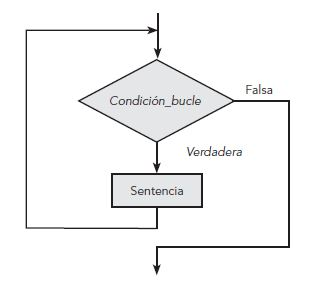
\includegraphics[scale=0.4]{flujoWhile.JPG}\vspace{-5mm}\end{center}
    \justify
    \hspace{5mm}
    El diagrama indica que la ejecución de la sentencia se repite mientras la condición permanece verdadera y termina cuando se hace falsa. También que la condición del ciclo se evalúa antes de ejecutar el cuerpo del ciclo, si esta condición es inicialmente falsa, el cuerpo del ciclo no se ejecutará. En otras palabras, el cuerpo de un bucle while se ejecutará cero o más veces.
\end{frame}


% - - - - - - - - - - - - - - - - - - - - - Slide 07 - - - - - - - - - - - - - - - - - - - - - - -
\begin{frame}[fragile]{Tipos de ciclos}

    \begin{center}\textbf{Ejemplos}\end{center}
    \begin{columns}
        \begin{column}{0.5 \textwidth}
            El siguien ciclo cuenta hasta 10
        \begin{lstlisting}
int x = 0;
while( x < 10 )
    printf("X: %d\n", x++);
\end{lstlisting}
        \end{column}
        \begin{column}{0.4 \textwidth}
    Visualizar n asteriscos
    \begin{lstlisting}
contador = 0;
while( contador < n )
{
    printf(" * ");
    contador++;
}/*Fin del while*/
\end{lstlisting}
        \end{column}
    \end{columns}
\end{frame}

% - - - - - - - - - - - - - - - - - - - - - Slide 08 - - - - - - - - - - - - - - - - - - - - - - -
\begin{frame}[fragile]{Tipos de ciclos}
    \begin{center}
        \textbf{Ciclo Infinito}
    \end{center}
    \justify
    Si la variable de control no se actualiza el ciclo se ejecutará “siempre” (ciclo infinito). Un ciclo infinito (sin terminación) se produce cuando la condición del permanece y no se hace falsa en ninguna iteración.
    \vspace{-2mm}
\begin{center}
    \begin{tabular}{c}
            \begin{lstlisting}
/* bucle infinito */
contador = 1;
while (contador < 100)
{
    printf("%d \n", contador);
    contador--;
}
\end{lstlisting}
    \end{tabular}
\end{center}
\end{frame}



% - - - - - - - - - - - - - - - - - - - - - Slide 09 - - - - - - - - - - - - - - - - - - - - - - -
\begin{frame}[fragile]{Tipos de ciclos}
\begin{center}
    \textbf{CICLO DE MUESTRA CON \textit{WHILE}}
\end{center}
\lstinputlisting[style=customc]{codigos/ciclos/cicloMuestra.c}
\end{frame}



% - - - - - - - - - - - - - - - - - - - - - Slide 10 - - - - - - - - - - - - - - - - - - - - - - -
\begin{frame}{Tipos de ciclos}
content...
\end{frame}



% - - - - - - - - - - - - - - - - - - - - - Slide 11 - - - - - - - - - - - - - - - - - - - - - - -
\begin{frame}{Tipos de ciclos}
content...
\end{frame}



% - - - - - - - - - - - - - - - - - - - - - Slide 12 - - - - - - - - - - - - - - - - - - - - - - -
\begin{frame}{Tipos de ciclos}
content...
\end{frame}